% SOURCE: RG_signed_reanalysis_REFIX20260801.json :: bundles.{Qwen2.5-14B_L36,Llama-3.2-1B_L12}.cells.g*.frac_drop_negative (14B 0.665@g20, 1B 0.000@g20)
% !TEX encoding = UTF-8 Unicode
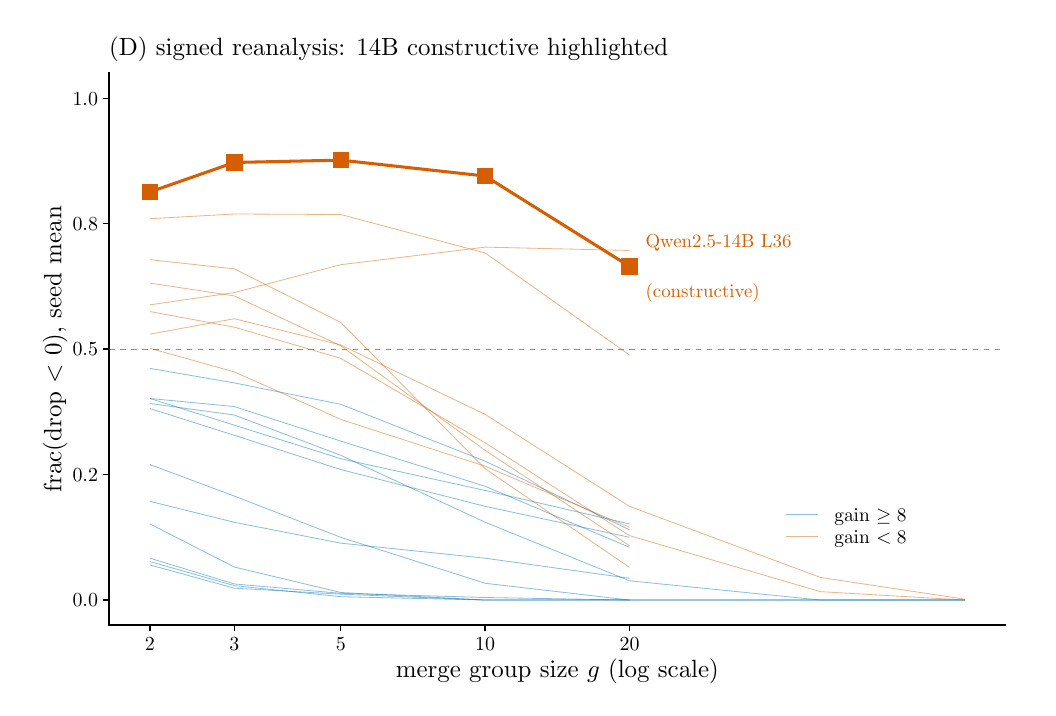
\begin{tikzpicture}[x=1pt,y=1pt]
\definecolor{fillColor}{RGB}{255,255,255}
\path[use as bounding box,fill=fillColor,fill opacity=0.00] (0,0) rectangle (361.35,238.49);
\begin{scope}
\path[clip] (  0.00,  0.00) rectangle (361.35,238.49);
\definecolor{drawColor}{RGB}{255,255,255}
\definecolor{fillColor}{RGB}{255,255,255}

\path[draw=drawColor,line width= 0.5pt,line join=round,line cap=round,fill=fillColor] (  0.00,  0.00) rectangle (361.35,238.49);
\end{scope}
\begin{scope}
\path[clip] ( 29.45, 22.61) rectangle (353.35,222.04);
\definecolor{fillColor}{RGB}{255,255,255}

\path[fill=fillColor] ( 29.45, 22.61) rectangle (353.35,222.04);
\definecolor{drawColor}{gray}{0.55}

\path[draw=drawColor,line width= 0.3pt,dash pattern=on 2pt off 2pt ,line join=round] ( 29.45,122.32) -- (353.35,122.32);
\definecolor{drawColor}{RGB}{0,114,178}

\path[draw=drawColor,draw opacity=0.45,line width= 0.3pt,line join=round] ( 44.17,104.50) --
	( 74.69, 94.85) --
	(113.14, 82.74) --
	(165.31, 71.26) --
	(217.48, 59.17);

\path[draw=drawColor,draw opacity=0.45,line width= 0.3pt,line join=round] ( 44.17, 67.33) --
	( 74.69, 59.75) --
	(113.14, 52.22) --
	(165.31, 46.78) --
	(217.48, 39.53);
\definecolor{drawColor}{RGB}{213,94,0}

\path[draw=drawColor,draw opacity=0.45,line width= 0.3pt,line join=round] ( 44.17,169.46) --
	( 74.69,171.16) --
	(113.14,170.98) --
	(165.31,157.08) --
	(217.48,120.21);

\path[draw=drawColor,draw opacity=0.45,line width= 0.3pt,line join=round] ( 44.17,138.34) --
	( 74.69,142.78) --
	(113.14,152.84) --
	(165.31,159.19) --
	(217.48,157.98);
\definecolor{drawColor}{RGB}{0,114,178}

\path[draw=drawColor,draw opacity=0.45,line width= 0.3pt,line join=round] ( 44.17, 80.62) --
	( 74.69, 69.22) --
	(113.14, 54.33) --
	(165.31, 37.72) --
	(217.48, 31.67);

\path[draw=drawColor,draw opacity=0.45,line width= 0.3pt,line join=round] ( 44.17, 46.78) --
	( 74.69, 37.48) --
	(113.14, 34.09) --
	(165.31, 32.58) --
	(217.48, 31.67) --
	(286.45, 31.67) --
	(338.63, 31.67);

\path[draw=drawColor,draw opacity=0.45,line width= 0.3pt,line join=round] ( 44.17, 44.36) --
	( 74.69, 35.95) --
	(113.14, 33.79) --
	(165.31, 31.67) --
	(217.48, 31.67) --
	(286.45, 31.67) --
	(338.63, 31.67);

\path[draw=drawColor,draw opacity=0.45,line width= 0.3pt,line join=round] ( 44.17, 59.17) --
	( 74.69, 43.58) --
	(113.14, 34.39) --
	(165.31, 31.67) --
	(217.48, 31.67) --
	(286.45, 31.67) --
	(338.63, 31.67);

\path[draw=drawColor,draw opacity=0.45,line width= 0.3pt,line join=round] ( 44.17, 45.57) --
	( 74.69, 36.86) --
	(113.14, 32.88) --
	(165.31, 31.67) --
	(217.48, 31.67);

\path[draw=drawColor,draw opacity=0.45,line width= 0.3pt,line join=round] ( 44.17,104.50) --
	( 74.69,101.57) --
	(113.14, 89.09) --
	(165.31, 72.77) --
	(217.48, 50.71);

\path[draw=drawColor,draw opacity=0.45,line width= 0.3pt,line join=round] ( 44.17,100.87) --
	( 74.69, 91.19) --
	(113.14, 78.81) --
	(165.31, 65.52) --
	(217.48, 54.33);
\definecolor{drawColor}{RGB}{213,94,0}

\path[draw=drawColor,draw opacity=0.45,line width= 0.3pt,line join=round] ( 44.17,154.66) --
	( 74.69,151.33) --
	(113.14,131.99) --
	(165.31, 79.11) --
	(217.48, 43.46);
\definecolor{drawColor}{RGB}{0,114,178}

\path[draw=drawColor,draw opacity=0.45,line width= 0.3pt,line join=round] ( 44.17,102.68) --
	( 74.69, 98.52) --
	(113.14, 83.95) --
	(165.31, 59.77) --
	(217.48, 38.62) --
	(286.45, 31.67) --
	(338.63, 31.67);
\definecolor{drawColor}{RGB}{213,94,0}

\path[draw=drawColor,draw opacity=0.45,line width= 0.3pt,line join=round] ( 44.17,135.92) --
	( 74.69,130.26) --
	(113.14,119.00) --
	(165.31, 88.48) --
	(217.48, 54.94) --
	(286.45, 34.69) --
	(338.63, 31.67);

\path[draw=drawColor,draw opacity=0.45,line width= 0.3pt,line join=round] ( 44.17,127.76) --
	( 74.69,133.31) --
	(113.14,123.84) --
	(165.31, 98.75) --
	(217.48, 65.52) --
	(286.45, 39.83) --
	(338.63, 31.97);
\definecolor{drawColor}{RGB}{0,114,178}

\path[draw=drawColor,draw opacity=0.45,line width= 0.3pt,line join=round] ( 44.17,115.37) --
	( 74.69,110.12) --
	(113.14,102.38) --
	(165.31, 81.83) --
	(217.48, 57.05);
\definecolor{drawColor}{RGB}{213,94,0}

\path[draw=drawColor,draw opacity=0.45,line width= 0.3pt,line join=round] ( 44.17,146.20) --
	( 74.69,141.56) --
	(113.14,123.53) --
	(165.31, 85.76) --
	(217.48, 51.31);

\path[draw=drawColor,draw opacity=0.45,line width= 0.3pt,line join=round] ( 44.17,122.63) --
	( 74.69,114.09) --
	(113.14, 96.94) --
	(165.31, 80.02) --
	(217.48, 57.96);
\definecolor{drawColor}{RGB}{213,94,0}

\path[draw=drawColor,line width= 1.1pt,line join=round] ( 44.17,179.13) --
	( 74.69,189.78) --
	(113.14,190.62) --
	(165.31,184.88) --
	(217.48,152.24);
\definecolor{fillColor}{RGB}{213,94,0}

\path[fill=fillColor] ( 41.20,176.17) --
	( 47.14,176.17) --
	( 47.14,182.10) --
	( 41.20,182.10) --
	cycle;

\path[fill=fillColor] ( 71.72,186.81) --
	( 77.66,186.81) --
	( 77.66,192.75) --
	( 71.72,192.75) --
	cycle;

\path[fill=fillColor] (110.17,187.65) --
	(116.11,187.65) --
	(116.11,193.59) --
	(110.17,193.59) --
	cycle;

\path[fill=fillColor] (162.34,181.91) --
	(168.28,181.91) --
	(168.28,187.84) --
	(162.34,187.84) --
	cycle;

\path[fill=fillColor] (214.52,149.27) --
	(220.45,149.27) --
	(220.45,155.21) --
	(214.52,155.21) --
	cycle;

\node[text=drawColor,anchor=base west,inner sep=0pt, outer sep=0pt, scale=  0.68] at (223.28,158.95) {Qwen2.5-14B L36};

\node[text=drawColor,anchor=base west,inner sep=0pt, outer sep=0pt, scale=  0.68] at (223.28,140.82) {(constructive)};
\end{scope}
\begin{scope}
\path[clip] (  0.00,  0.00) rectangle (361.35,238.49);
\definecolor{drawColor}{RGB}{0,0,0}

\path[draw=drawColor,line width= 0.5pt,line join=round,line cap=rect] ( 29.45, 22.61) --
	( 29.45,222.04);
\end{scope}
\begin{scope}
\path[clip] (  0.00,  0.00) rectangle (361.35,238.49);
\definecolor{drawColor}{RGB}{0,0,0}

\node[text=drawColor,anchor=base east,inner sep=0pt, outer sep=0pt, scale=  0.72] at ( 25.40, 29.19) {0.0};

\node[text=drawColor,anchor=base east,inner sep=0pt, outer sep=0pt, scale=  0.72] at ( 25.40, 74.52) {0.2};

\node[text=drawColor,anchor=base east,inner sep=0pt, outer sep=0pt, scale=  0.72] at ( 25.40,119.85) {0.5};

\node[text=drawColor,anchor=base east,inner sep=0pt, outer sep=0pt, scale=  0.72] at ( 25.40,165.17) {0.8};

\node[text=drawColor,anchor=base east,inner sep=0pt, outer sep=0pt, scale=  0.72] at ( 25.40,210.50) {1.0};
\end{scope}
\begin{scope}
\path[clip] (  0.00,  0.00) rectangle (361.35,238.49);
\definecolor{drawColor}{RGB}{0,0,0}

\path[draw=drawColor,line width= 0.5pt,line join=round] ( 27.20, 31.67) --
	( 29.45, 31.67);

\path[draw=drawColor,line width= 0.5pt,line join=round] ( 27.20, 77.00) --
	( 29.45, 77.00);

\path[draw=drawColor,line width= 0.5pt,line join=round] ( 27.20,122.32) --
	( 29.45,122.32);

\path[draw=drawColor,line width= 0.5pt,line join=round] ( 27.20,167.65) --
	( 29.45,167.65);

\path[draw=drawColor,line width= 0.5pt,line join=round] ( 27.20,212.98) --
	( 29.45,212.98);
\end{scope}
\begin{scope}
\path[clip] (  0.00,  0.00) rectangle (361.35,238.49);
\definecolor{drawColor}{RGB}{0,0,0}

\path[draw=drawColor,line width= 0.5pt,line join=round,line cap=rect] ( 29.45, 22.61) --
	(353.35, 22.61);
\end{scope}
\begin{scope}
\path[clip] (  0.00,  0.00) rectangle (361.35,238.49);
\definecolor{drawColor}{RGB}{0,0,0}

\path[draw=drawColor,line width= 0.5pt,line join=round] ( 44.17, 20.36) --
	( 44.17, 22.61);

\path[draw=drawColor,line width= 0.5pt,line join=round] ( 74.69, 20.36) --
	( 74.69, 22.61);

\path[draw=drawColor,line width= 0.5pt,line join=round] (113.14, 20.36) --
	(113.14, 22.61);

\path[draw=drawColor,line width= 0.5pt,line join=round] (165.31, 20.36) --
	(165.31, 22.61);

\path[draw=drawColor,line width= 0.5pt,line join=round] (217.48, 20.36) --
	(217.48, 22.61);
\end{scope}
\begin{scope}
\path[clip] (  0.00,  0.00) rectangle (361.35,238.49);
\definecolor{drawColor}{RGB}{0,0,0}

\node[text=drawColor,anchor=base,inner sep=0pt, outer sep=0pt, scale=  0.72] at ( 44.17, 13.60) {2};

\node[text=drawColor,anchor=base,inner sep=0pt, outer sep=0pt, scale=  0.72] at ( 74.69, 13.60) {3};

\node[text=drawColor,anchor=base,inner sep=0pt, outer sep=0pt, scale=  0.72] at (113.14, 13.60) {5};

\node[text=drawColor,anchor=base,inner sep=0pt, outer sep=0pt, scale=  0.72] at (165.31, 13.60) {10};

\node[text=drawColor,anchor=base,inner sep=0pt, outer sep=0pt, scale=  0.72] at (217.48, 13.60) {20};
\end{scope}
\begin{scope}
\path[clip] (  0.00,  0.00) rectangle (361.35,238.49);
\definecolor{drawColor}{RGB}{0,0,0}

\node[text=drawColor,anchor=base,inner sep=0pt, outer sep=0pt, scale=  0.90] at (191.40,  3.75) {merge group size $g$ (log scale)};
\end{scope}
\begin{scope}
\path[clip] (  0.00,  0.00) rectangle (361.35,238.49);
\definecolor{drawColor}{RGB}{0,0,0}

\node[text=drawColor,rotate= 90.00,anchor=base,inner sep=0pt, outer sep=0pt, scale=  0.90] at ( 12.20,122.32) {frac(drop $<$ 0), seed mean};
\end{scope}
\begin{scope}
\path[clip] (  0.00,  0.00) rectangle (361.35,238.49);
\definecolor{fillColor}{RGB}{255,255,255}

\path[fill=fillColor] (272.54, 58.51) rectangle (287.00, 66.51);
\definecolor{drawColor}{RGB}{0,114,178}

\path[draw=drawColor,draw opacity=0.45,line width= 0.3pt,line join=round] (273.99, 62.51) -- (285.55, 62.51);
\end{scope}
\begin{scope}
\path[clip] (  0.00,  0.00) rectangle (361.35,238.49);
\definecolor{fillColor}{RGB}{255,255,255}

\path[fill=fillColor] (272.54, 50.51) rectangle (287.00, 58.51);
\definecolor{drawColor}{RGB}{213,94,0}

\path[draw=drawColor,draw opacity=0.45,line width= 0.3pt,line join=round] (273.99, 54.51) -- (285.55, 54.51);
\end{scope}
\begin{scope}
\path[clip] (  0.00,  0.00) rectangle (361.35,238.49);
\definecolor{drawColor}{RGB}{0,0,0}

\node[text=drawColor,anchor=base west,inner sep=0pt, outer sep=0pt, scale=  0.70] at (291.50, 60.09) {gain $\geq 8$};
\end{scope}
\begin{scope}
\path[clip] (  0.00,  0.00) rectangle (361.35,238.49);
\definecolor{drawColor}{RGB}{0,0,0}

\node[text=drawColor,anchor=base west,inner sep=0pt, outer sep=0pt, scale=  0.70] at (291.50, 52.09) {gain $< 8$};
\end{scope}
\begin{scope}
\path[clip] (  0.00,  0.00) rectangle (361.35,238.49);
\definecolor{drawColor}{RGB}{0,0,0}

\node[text=drawColor,anchor=base west,inner sep=0pt, outer sep=0pt, scale=  0.90] at ( 29.45,228.29) {(D) signed reanalysis: 14B constructive highlighted};
\end{scope}
\end{tikzpicture}
